\documentclass[tikz,border=2pt]{standalone}
\usepackage{tikz}
\usetikzlibrary{calc}

\begin{document}
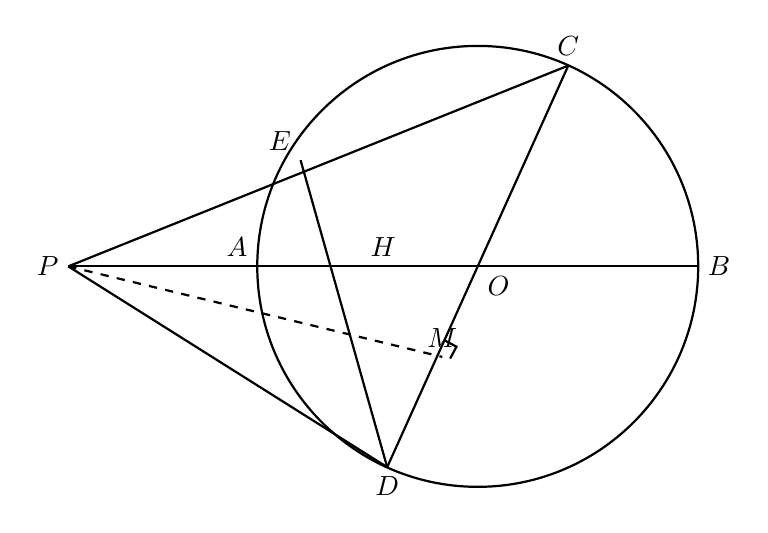
\begin{tikzpicture}[scale=1]
  % Circle
  \def\R{2.8}
  \coordinate (O) at (0,0);
  \draw[line width=0.8pt] (O) circle (\R);

  % Main points
  \coordinate (P) at (-5.2,0);
  \coordinate (A) at (-2.8,0);
  \coordinate (B) at (2.8,0);
  \coordinate (C) at (1.15,2.55);
  \coordinate (D) at (-1.15,-2.55);
  \coordinate (E) at (-2.25,1.35);

  % Horizontal secant
  \draw[line width=0.8pt] (P) -- (B);

  % Two secants from P
  \draw[line width=0.8pt] (P) -- (C);
  \draw[line width=0.8pt] (P) -- (D);

  % Chords
  \draw[line width=0.8pt] (E) -- (D);
  \draw[line width=0.8pt] (D) -- (C);

  % Dashed segment to H
  \coordinate (H) at (-0.45,-1.15);
  \draw[line width=0.8pt,dashed] (P) -- (H);

  % Right angle mark at H with respect to DC
  \coordinate (u) at ($(D)!0.58!(C)$);
  \draw[line width=0.8pt] ($(H)+(0.10,-0.02)$) -- ($(H)+(0.18,0.13)$) -- ($(H)+(0.03,0.21)$);

  % Point M on horizontal line
  \coordinate (M) at (-1.20,0);

  % Labels
  \node[left] at (P) {$P$};
  \node[above left] at (A) {$A$};
  \node[right] at (B) {$B$};
  \node[above] at (C) {$C$};
  \node[below] at (D) {$D$};
  \node[above left] at (E) {$E$};
  \node[below right] at (O) {$O$};

  % Swapped visible labels of H and M
  \node[above] at (H) {$M$};
  \node[above] at (M) {$H$};

\end{tikzpicture}
\end{document}
